%%%%%%%%%%%%%%%%%%%%%%% file template.tex %%%%%%%%%%%%%%%%%%%%%%%%%
%
% This is a general template file for the LaTeX package SVJour3
% for Springer journals.          Springer Heidelberg 2010/09/16
%
% Copy it to a new file with a new name and use it as the basis
% for your article. Delete % signs as needed.
%
% This template includes a few options for different layouts and
% content for various journals. Please consult a previous issue of
% your journal as needed.
%
%%%%%%%%%%%%%%%%%%%%%%%%%%%%%%%%%%%%%%%%%%%%%%%%%%%%%%%%%%%%%%%%%%%
%
% First comes an example EPS file -- just ignore it and
% proceed on the \documentclass line
% your LaTeX will extract the file if required
\begin{filecontents*}{example.eps}
%!PS-Adobe-3.0 EPSF-3.0
%%BoundingBox: 19 19 221 221
%%CreationDate: Mon Sep 29 1997
%%Creator: programmed by hand (JK)
%%EndComments
gsave
newpath
  20 20 moveto
  20 220 lineto
  220 220 lineto
  220 20 lineto
closepath
2 setlinewidth
gsave
  .4 setgray fill
grestore
stroke
grestore
\end{filecontents*}
%
\RequirePackage{fix-cm}
%
%\documentclass{svjour3}                     % onecolumn (standard format)
%\documentclass[smallcondensed]{svjour3}     % onecolumn (ditto)
%\documentclass[smallextended]{svjour3}       % onecolumn (second format)
\documentclass[twocolumn]{svjour3}          % twocolumn
%
\smartqed  % flush right qed marks, e.g. at end of proof
%
\usepackage{graphicx}
%
% \usepackage{mathptmx}      % use Times fonts if available on your TeX system
%
% insert here the call for the packages your document requires
%\usepackage{latexsym}
% etc.
%
% please place your own definitions here and don't use \def but
% \newcommand{}{}
%
% Insert the name of "your journal" with
% \journalname{}
%
\begin{document}

\title{STRUCTURAL DESIGN OF CARBON/EPOXY WIND TURBINE BLADE USING FLUID/STRUCTURE SIMULATION%\thanks{Grants or other notes
%about the article that should go on the front page should be
%placed here. General acknowledgments should be placed at the end of the article.}
}
%\subtitle{Do you have a subtitle?\\ If so, write it here}

%\titlerunning{Short form of title}        % if too long for running head

\author{Julian Sierra P \and Mariana Correa A        \and
        Valentina Villada Q %etc.
}

%\authorrunning{Short form of author list} % if too long for running head

\institute{Universidad Pontificia Bolivariana \at
              Campus de Laureles Circular 1 Nº 70-01 \\
              Tel.: +574-4488388\\
              Fax: +574-4488388\\
              \email{julian.sierra@upb.edu.co}           
           \and
           %Ecovias \at
              %second address
}

%\date{Received: date / Accepted: date}
% The correct dates will be entered by the editor


\maketitle

\begin{abstract}
This paper discusses the process of structural design of a wind turbine blade in carbon/epoxy. Two types of carbon fiber (unidirectional and woven) were mechanically characterized by standardized tests to obtain main mechanical properties of the composite.

An aerodynamic simulation was performed in order to obtain the pressure distribution profile of the blade, with a previously validated model, in order to carry out a fluid structure interaction simulation. It was obtained an optimum distribution which allowed balance between aerodynamic and the inertial loads, so that the geometry would not change or get deformed. Minimal deflection at the tip, equivalent to 3.11 cm and a total weight of 3.6 kg were obtained.%Insert your abstract here. Include keywords, PACS and mathematical
%subject classification numbers as needed.
\keywords{Structural Design\and Wind Turbine Blade\and Carbon/Epoxy\and Mechanical Characterization\and Fluid Structure Interaction\and Aerodynamic Loads\and Inertial Loads}
% \PACS{PACS code1 \and PACS code2 \and more}
% \subclass{MSC code1 \and MSC code2 \and more}
\end{abstract}

\section{Introduction}
\label{intro}
Nowadays the development of renewable energies has obtained mayor importance, this carries to growth of energy industries, such as the eolic. By the end of last year, approximately 268000 wind turbines operated around the world \cite{gwec}, becoming in focus of studies and analyses in their aerodynamic behavior as well as structural, in order to search the best performance characteristics according to the operation conditions.

The use of composite materials in its manufacture provides excellent mechanical properties, resistance to environmental conditions, low weight and non-conventional shapes possibilities, allowing less complex manufacture processes \cite{Mish} .

This paper presents the structural design of a low-speed, horizontal axis, bioinspired wind turbine blade, which uses a composite material formed by carbon/epoxy laminates. The design is achieved through a Fluid Structure Interaction simulation of the blade. 

In order to determine materials’ mechanical properties (simulation’s input parameters), carbon/epoxy laminates are characterized. The combination of this series of activities, allows to carry out an interactive simulation to obtain an effective design where aerodynamic loads counter inertial loads, avoiding distortions of the geometry during the operation that could affect its performance.  

%Your text comes here. Separate text sections with
\section{Theoretical framework}
The composite materials present huge advantages regarding traditional ones used in aerospace. Its specific modulus and specific strength are comparatively high, allowing the weight reduction in components. The anisotropy characteristic of the material makes possible the introduction of properties such as strength and stiffness, when the product requires it \cite{hull}.

The carbon fiber breaks fragile to tension with relatively small strains comparing with metal alloys. It can be 13 times more resistant in tension, 4 times more rigid and 1.5 times lighter than the aluminum \cite{lin}. Epoxy resins offer the best mechanical properties and great performance at high temperatures. 
\label{sec:1}
%Text with citations \cite{RefB} and \cite{RefJ}.
%\subsection{Mechanical properties}
For an anisotropic material, the engineering constants are defined as: Young Modulus $(E_1,E_2,E_3)$, shear modulus $(G_1_2,G_2_3,G_3_1)$ and Poisson ratio $(v_1_2)$. Where, $1$ is equivalent to $x$, $2$ to the $y$ direction, and $3$ to the $z$ direction.

\begin{figure}
% Use the relevant command to insert your figure file.
% For example, with the graphicx package use
  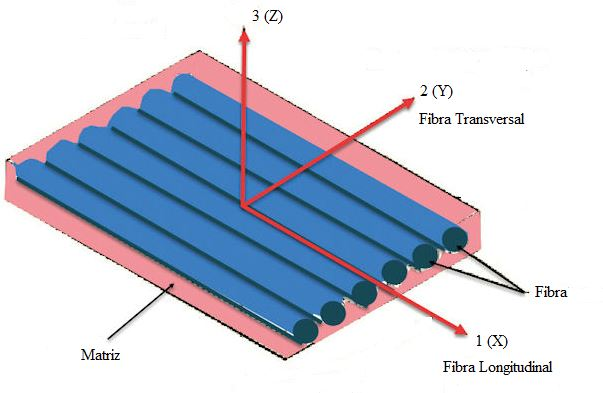
\includegraphics[width=0.75\textwidth]{direction}
% figure caption is below the figure
\caption{Directions in the laminate}
\label{fig:dl}       % Give a unique label
\end{figure}

There are three failure modes for interlaminar fracture: Mode I (opening), mode II (shearing) and mode III (tearing). The theoretical modeling of delamination in composite materials can be made according to Linear-Elastic Fracture Mechanics . Each mode has an associated value of fracture toughness: $G_I_C, G_I_I_C, G_I_I_I_C$ defined as the energy available for the advance of crack per unit area or Energy Release Rate.

The tensile test consists in subjecting the specimen to a tensile load along its main axis, causing an elongation of the specimen in that direction until it reaches the break point. In the  shear plane test, a tensile test is performed on a laminate $[± 45 °]$ locating two strain gages, one in longitudinal direction and another one in transverse direction (Tsai y Miravete 1988).

The most common used test to evaluate the interlaminar fracture toughness in mode I is Double Cantilever Beam, where opening forces are applied on the specimen by means of hinges or tabs attached to one end of the specimen. In the test Mixed Mode I / II, an apparatus that splits the load into two: one of them is applied via tabs located at the ends of the delaminated section of the specimen, and the other is applied via rollers which rest against the region not delaminated. 

%\subsection{Failure Criteria}
The failure criteria are intended to predict the failure of the sheet. Following the approach used in this paper is exposed. 

Theory of maximum deformation: The failure occurs when any component of strain along the principal axes of the material exceeds or equals the experimental strain value to which the failure occurs and one of the following equations are true:
\begin{equation}
\varepsilon_1=\varepsilon_1_t^u,  si  \varepsilon_1>0  o  \varepsilon_1_c^u,  si  \varepsilon_1<0
\end{equation}
%\varepsilon_2=\varepsilon_2_t^u, si \varepsilon_2_c^u, si \varepsilon_1<0  
%\end{equation}
%\end{equation}
%\label{sec:2}
%as required. Don't forget to give each section
%and subsection a unique label (see Sect.~\ref{sec:1}).
%\paragraph{Paragraph headings} Use paragraph headings as needed.
%\begin{equation}
%a^2+b^2=c^2
%\end{equation}

Where , $\varepsilon_1, \varepsilon_2$ represent the normal strain and $\gamma_4, \gamma_5, \gamma_6$ shear strains in the point of interest; $c, t$, indicate compressive and tensile respectively,  these should be always positive.

%\subsection{Wind Turbines}
A wind turbine is a device which uses the power of the wind passing through its blades to cause a moment that moves the rotor shaft, transforming kinetic energy into electricity. The horizontal axis turbines are facing the wind and its axis of rotation is parallel to the ground. The energy obtained in a wind turbine is determined by the energy of the wind passing through the rotor, which depends on the air density, wind speed and swept area by the blades.

\section{State of the art}
Some researchers have developed methods for aerodynamic and power analysis of wind turbines. In a NREL (National Renewable Energy Laboratory) technical report, the geometry of a conventional wind turbine and the results obtained when tested in the wind tunnel (Hand, et al 2001) is presented; these values are then used as reference by Sørensen et al for comparison with those resulting from Computational Fluid Dynamics analysis and demonstrates the capacity of the software tool (Sørensen, and Schreck Michelsen 2002). Also, Lawson et al, presented a methodology for aerodynamic simulation where meshing characteristics and control volume adequate for analysis are discussed in more depth (Lawson, Li and DC 2011).

A research performed by Cárdenas et al, presents the numerical validation of Thin-Walled Beam model with finite elements for a wind turbine blade. One of the most advanced formulations which are achieved coupling effects of nonlinearity, arbitrary cross sections and anisotropic material, is the Variational Asymtotic Beam Sectional Analysis, which provides good results of stress / strain on finite element validations of models in three dimensions (Cardenas and others 2012).

Vasjaliya and Gangadharan developed a Fluid Structure Interaction simulation of a wind turbine blade to optimize it. The aerodynamic results of the blade obtained are transferred to the structural analysis module to calculate the constraints, strains and stresses which are taken as output parameters to optimize the iterative process to achieve the best performance design (Vasjaliya and Gangadharan, University of Florida 2012).

% For one-column wide figures use
%\begin{figure}
% Use the relevant command to insert your figure file.
% For example, with the graphicx package use
 % 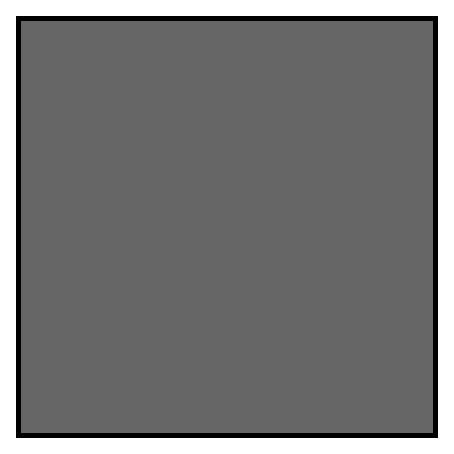
\includegraphics{example.eps}
% figure caption is below the figure
%\caption{Please write your figure caption here}
%\label{fig:1}       % Give a unique label
%\end{figure}
%
% For two-column wide figures use
%\begin{figure*}
% Use the relevant command to insert your figure file.
% For example, with the graphicx package use
  %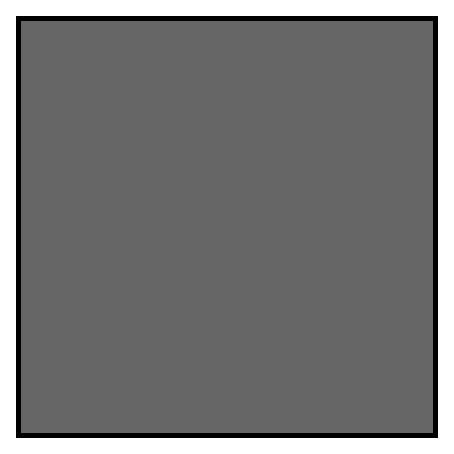
\includegraphics[width=0.75\textwidth]{example.eps}
% figure caption is below the figure
%\caption{Please write your figure caption here}
%\label{fig:2}       % Give a unique label
%\end{figure*}
%
% For tables use
%\begin{table}
% table caption is above the table
%\caption{Please write your table caption here}
%\label{tab:1}       % Give a unique label
% For LaTeX tables use
%\begin{tabular}{lll}
%\hline\noalign{\smallskip}
%first & second & third  \\
%\noalign{\smallskip}\hline\noalign{\smallskip}
%number & number & number \\
%number & number & number \\
%\noalign{\smallskip}\hline
%\end{tabular}
%\end{table}


%\begin{acknowledgements}
%If you'd like to thank anyone, place your comments here
%and remove the percent signs.
%\end{acknowledgements}

% BibTeX users please use one of
%\bibliographystyle{spbasic}      % basic style, author-year citations
%\bibliographystyle{spmpsci}      % mathematics and physical sciences
%\bibliographystyle{spphys}       % APS-like style for physics
%\bibliography{}   % name your BibTeX data base

% Non-BibTeX users please use
\begin{thebibliography}{}
%
% and use \bibitem to create references. Consult the Instructions
% for authors for reference list style.
%
%\bibitem{RefJ}
% Format for Journal Reference
%Author, Article title, Journal, Volume, page numbers (year)
% Format for books
%\bibitem{RefB}
Author, Book title, page numbers. Publisher, place (year)
% etc
\end{thebibliography}

\end{document}
% end of file template.tex

